\chapter{Infrared spectra}
\label{chap:irSpectra}

In this chapter we present some general observations and discuss with more detail the infrared-active exctitations.
We start with section \ref{sec:classification} describing the general nature of the different excitations. 
In section \ref{sec:irSpectra} we analyze some features that should be present in the infrared spectra followed, in section \ref{sec:irIsotopicShifts}, by a description of the effects that the isotopic $^{16}$O$\rightarrow ^{18}$O substitution has in the spectra. 
Finally we conclude in section \ref{sec:irPhononProj} with some observations about the projections into the phonon coordinates of these infrared-active states.
We defer to appendix \ref{chap:comp_details} some specific details about the calculations, such as the algorithm used and the numerical errors introduced by the truncation in the basis.

\section{Classification of the excitations}
\label{sec:classification}

As previously noted in section \ref{sec:hamiltonian-and-basis}, only for zero charge-lattice couplings the eigenstates of the many-body Hamiltonian (\ref{eq:full-hamiltonian}) can be described as a direct product of an electronic and a phononic state, that is, eigenstates of the full hamiltonian $H$ are products of eigenstates of $H_{el}$ and $H_{ph}$ respectively.
In this uncoupled scenatio the phonon number opreators $b_Rb^\dagger_R$ and $b_{ir}b^\dagger_{ir}$ have integer values with zero dispersion.
Increasing the value of the coupling parameters produces eigenstates with different mean phonon values and some finite dispersion producing eigenstates that can not be separated as a product of phononic and electronic states.
However, the deviation from this behaviour is smooth in the coupling parameter $\lambda_{ir}$.
That is, a hamiltonian with a small $\lambda_{ir}$ value will have only slighty different eigenstates from the uncoupled hamiltonian.
This slightly mixed eigenstates in the small couping regime can be thought of as largely \textit{phononic} or \textit{electronic} in nature.
For larger coupling values the eigenstates are very different from their uncoupled counterparts.
As an illustration of this we show, in figure \ref{fig:electr-proj}, the first electronic excitation for different $\lambda_{ir}$ values, $\psi_{el}(\lambda_{ir})$ projected with itself for the uncoupled system, $\psi_{el}(\lambda_{ir}=0)$.
From this projection we can see that for small coupling values $\psi_{el}$ remains largely unchanged, that is, it remains \textit{electronic} in nature.
In the middle coupling regime the change is the strongest with the projection approaching asymptotically to zero at large couplings.
The vertical line in \ref{fig:electr-proj} at $\lambda_{ir}=0.1263$ eV, as discussed in section \ref{sec:grd-phonon-proj}, represents the $\lambda_{ir}$ value that reproduces the experimentally observed cluster distortion of 0.13 \AA.
At this coupling value the electronic eigenstate has a projection with its uncoupled counterpart near 0.75 which indicates that, although it has been somewhat changed, it remains mostly \textit{electronic} in nature.
Similar observations can be made for the rest of the excitations in this model.
For this reason even though the eigenstates, for finite charge-lattice couplings, are not strictly electronic or phononic we will continue to refer to them as such since that interpretation remains useful in the regime of interest to us.
Given the possibility of making such a distinction for the different excitations we will discuss \textit{phononic} and \textit{electronic} excitations separatedly in this and the next chapters respectively. 
%
\begin{figure}[ht]
  \centering
  % GNUPLOT: LaTeX picture with Postscript
\begingroup
  \makeatletter
  \providecommand\color[2][]{%
    \GenericError{(gnuplot) \space\space\space\@spaces}{%
      Package color not loaded in conjunction with
      terminal option `colourtext'%
    }{See the gnuplot documentation for explanation.%
    }{Either use 'blacktext' in gnuplot or load the package
      color.sty in LaTeX.}%
    \renewcommand\color[2][]{}%
  }%
  \providecommand\includegraphics[2][]{%
    \GenericError{(gnuplot) \space\space\space\@spaces}{%
      Package graphicx or graphics not loaded%
    }{See the gnuplot documentation for explanation.%
    }{The gnuplot epslatex terminal needs graphicx.sty or graphics.sty.}%
    \renewcommand\includegraphics[2][]{}%
  }%
  \providecommand\rotatebox[2]{#2}%
  \@ifundefined{ifGPcolor}{%
    \newif\ifGPcolor
    \GPcolortrue
  }{}%
  \@ifundefined{ifGPblacktext}{%
    \newif\ifGPblacktext
    \GPblacktextfalse
  }{}%
  % define a \g@addto@macro without @ in the name:
  \let\gplgaddtomacro\g@addto@macro
  % define empty templates for all commands taking text:
  \gdef\gplbacktext{}%
  \gdef\gplfronttext{}%
  \makeatother
  \ifGPblacktext
    % no textcolor at all
    \def\colorrgb#1{}%
    \def\colorgray#1{}%
  \else
    % gray or color?
    \ifGPcolor
      \def\colorrgb#1{\color[rgb]{#1}}%
      \def\colorgray#1{\color[gray]{#1}}%
      \expandafter\def\csname LTw\endcsname{\color{white}}%
      \expandafter\def\csname LTb\endcsname{\color{black}}%
      \expandafter\def\csname LTa\endcsname{\color{black}}%
      \expandafter\def\csname LT0\endcsname{\color[rgb]{1,0,0}}%
      \expandafter\def\csname LT1\endcsname{\color[rgb]{0,1,0}}%
      \expandafter\def\csname LT2\endcsname{\color[rgb]{0,0,1}}%
      \expandafter\def\csname LT3\endcsname{\color[rgb]{1,0,1}}%
      \expandafter\def\csname LT4\endcsname{\color[rgb]{0,1,1}}%
      \expandafter\def\csname LT5\endcsname{\color[rgb]{1,1,0}}%
      \expandafter\def\csname LT6\endcsname{\color[rgb]{0,0,0}}%
      \expandafter\def\csname LT7\endcsname{\color[rgb]{1,0.3,0}}%
      \expandafter\def\csname LT8\endcsname{\color[rgb]{0.5,0.5,0.5}}%
    \else
      % gray
      \def\colorrgb#1{\color{black}}%
      \def\colorgray#1{\color[gray]{#1}}%
      \expandafter\def\csname LTw\endcsname{\color{white}}%
      \expandafter\def\csname LTb\endcsname{\color{black}}%
      \expandafter\def\csname LTa\endcsname{\color{black}}%
      \expandafter\def\csname LT0\endcsname{\color{black}}%
      \expandafter\def\csname LT1\endcsname{\color{black}}%
      \expandafter\def\csname LT2\endcsname{\color{black}}%
      \expandafter\def\csname LT3\endcsname{\color{black}}%
      \expandafter\def\csname LT4\endcsname{\color{black}}%
      \expandafter\def\csname LT5\endcsname{\color{black}}%
      \expandafter\def\csname LT6\endcsname{\color{black}}%
      \expandafter\def\csname LT7\endcsname{\color{black}}%
      \expandafter\def\csname LT8\endcsname{\color{black}}%
    \fi
  \fi
  \setlength{\unitlength}{0.0500bp}%
  \begin{picture}(6802.00,3968.00)%
    \gplgaddtomacro\gplbacktext{%
      \colorrgb{0.31,0.31,0.31}%
      \put(1078,751){\makebox(0,0)[r]{\strut{}\scriptsize 0}}%
      \colorrgb{0.31,0.31,0.31}%
      \put(1078,1313){\makebox(0,0)[r]{\strut{}\scriptsize 0.2}}%
      \colorrgb{0.31,0.31,0.31}%
      \put(1078,1876){\makebox(0,0)[r]{\strut{}\scriptsize 0.4}}%
      \colorrgb{0.31,0.31,0.31}%
      \put(1078,2438){\makebox(0,0)[r]{\strut{}\scriptsize 0.6}}%
      \colorrgb{0.31,0.31,0.31}%
      \put(1078,3000){\makebox(0,0)[r]{\strut{}\scriptsize 0.8}}%
      \colorrgb{0.31,0.31,0.31}%
      \put(1078,3562){\makebox(0,0)[r]{\strut{}\scriptsize 1}}%
      \colorrgb{0.31,0.31,0.31}%
      \put(1257,484){\makebox(0,0){\strut{}\scriptsize 0}}%
      \colorrgb{0.31,0.31,0.31}%
      \put(1669,484){\makebox(0,0){\strut{}\scriptsize 0.02}}%
      \colorrgb{0.31,0.31,0.31}%
      \put(2081,484){\makebox(0,0){\strut{}\scriptsize 0.04}}%
      \colorrgb{0.31,0.31,0.31}%
      \put(2493,484){\makebox(0,0){\strut{}\scriptsize 0.06}}%
      \colorrgb{0.31,0.31,0.31}%
      \put(2904,484){\makebox(0,0){\strut{}\scriptsize 0.08}}%
      \colorrgb{0.31,0.31,0.31}%
      \put(3316,484){\makebox(0,0){\strut{}\scriptsize 0.1}}%
      \colorrgb{0.31,0.31,0.31}%
      \put(3728,484){\makebox(0,0){\strut{}\scriptsize 0.12}}%
      \colorrgb{0.31,0.31,0.31}%
      \put(4140,484){\makebox(0,0){\strut{}\scriptsize 0.14}}%
      \colorrgb{0.31,0.31,0.31}%
      \put(4552,484){\makebox(0,0){\strut{}\scriptsize 0.16}}%
      \colorrgb{0.31,0.31,0.31}%
      \put(4964,484){\makebox(0,0){\strut{}\scriptsize 0.18}}%
      \colorrgb{0.31,0.31,0.31}%
      \put(5375,484){\makebox(0,0){\strut{}\scriptsize 0.2}}%
      \colorrgb{0.31,0.31,0.31}%
      \put(5787,484){\makebox(0,0){\strut{}\scriptsize 0.22}}%
      \colorrgb{0.31,0.31,0.31}%
      \put(6199,484){\makebox(0,0){\strut{}\scriptsize 0.24}}%
      \csname LTb\endcsname%
      \put(176,2227){\rotatebox{-270}{\makebox(0,0){\strut{}$\left|\braket{\psi (\lambda_{ir}=0)}{\psi (\lambda_{ir})}\right|$}}}%
      \put(3831,154){\makebox(0,0){\strut{}$\lambda_{ir}$ (eV)}}%
      \put(3934,3467){\makebox(0,0)[l]{\strut{}\scriptsize$\lambda_{ir}=0.1263$}}%
    }%
    \gplgaddtomacro\gplfronttext{%
    }%
    \gplbacktext
    \put(0,0){\includegraphics{images/electrProj}}%
    \gplfronttext
  \end{picture}%
\endgroup

  \caption[Projection of the first \textit{electronic} state with itself at $\lambda_{ir}=0$.]
  {Projection of the first \textit{electronic} state with itself at $\lambda_{ir}=0$.
    The vertical line denotes the experimentally relevant value $\lambda_{ir}=0.1263$ eV.}
  \label{fig:electr-proj}
\end{figure}

Since we are setting the charge-lattice coupling parameter to the symmetrical (Raman) vibrational mode ($\lambda_R$) as zero and these excitations are unchanged by an increase in $\lambda_{ir}$ all excitations will have a definite eigenvalue for the Raman number operator $b_R^\dagger b_R$. 
An excitation which, at $\lambda_{ir}=0$, has an eigenvalue of zero for the infrared number operator $b_{ir}^\dagger b_{ir}$ and for the electronic part of the hamiltonian $H_{el}$ (i.e. a pure \textit{Raman} excitation with no other components) will remain completely unchanged with a variation of $\lambda_{ir}$.
We will omit any discussion about these excitations and ignore them for the rest of this thesis. 


\section{Infrared spectra}
\label{sec:irSpectra}

The Peierls-Hubbard model (\ref{eq:full-hamiltonian}) applied to the O(4)-Cu(1)-O(4) cluster in YBa$_2$Cu$_3$O$_7$ should be able to predict some features of the c-axis infrared spectra by looking at the infrared-active excitations.
It should be noted that, since the coupling $\lambda_{ir}$ can be varied smoothly, the hamiltonian eigenstates will not change parity as a function of $\lambda_{ir}$.
Given that an excitation is infrared-active when it has an opposing parity to the ground state, it follows that an infrared-active excitation at $\lambda_{ir}=0$ will remain active across all the $\lambda_{ir}$ domain.
Since we are modelling the asymmetric vibrational (infared) mode in the O(4)-Cu(1)-O(4) cluster as an harmonic oscillator, it can be concluded that the infrared-active excitations, for any $\lambda_{ir}$, will be those that, at $\lambda_{ir}=0$, have an \textit{odd} number of phonons.

Figure \ref{fig:irSpectra} shows the infrared excitations for a representative range of $\lambda_{ir}$ values.
For $\lambda_{ir}=0$ we have the excitations corresponding to the phononic part of the hamiltonian.
As can be observed, the behaviour of each excitation depends on the number of infrared phonons at zero coupling.
The number of Raman phonons only displaces the excitation in multiples of $\omega_R=500$ cm$^{-1}$.
That is, all the red lines in Fig. \ref{fig:irSpectra} correspond to one infrared phonon and, in ascending order, have zero, one and two Raman phonons.
This is similarly true for the excitations with two (green lines) and three (blue lines) infrared phonons.
Notice that the excitations with two infrared phonons are not infrared-active since they have the same symmetry as the ground state.
%
\begin{figure}[ht]
  \centering
  \input{images/irSpectra}
  \caption[Infrared-active excitations as a function of electron-lattice coupling.]
  {Infrared-active excitations as a function of electron-lattice coupling.
  The red, green and blue lines denote excitations which, initially, have one, two and three infrared phonons respectively.
  The horizontal dashed line is placed at the first infared-active excitation $\omega_i=612.4$ cm$^{-1}$ as a guide to the eye.}
  \label{fig:irSpectra}
\end{figure}

In general, the infrared excitations decrease in energy with $\lambda_{ir}$ reaching asymptotically a lower value for large couplings.
The excitations with one infrared phonon decrease in energy converging to ($0,\omega_R,2\omega_R\ldots$).
However the excitations with two and three infrared phonons converge to ($\omega_{ir},2\omega_{ir},3\omega_{ir}\ldots$).
This recovery of an harmonic behaviour at large $\lambda_{ir}$ can be interpreted as a renormalization of the oscillations with a displaced equilibrium position.

The infrared spectra at $\lambda_{ir}=0$ eV and at the relevant coupling, $\lambda_{ir}=0.1263$ eV, is similar albeit with some noticeable differences.
The peak centered at 612.4 cm$^{-1}$ seems to be slightly shifted to 641.4 cm$^{-1}$ with an asymetry produced by the excitation with three infrared phonons at 774.2 cm$^{-1}$ (see inset of Fig. 2 in \cite{MustredeLeon1992} and Fig. 2 in \cite{Salkola1994}).
It should be noted that calculations using a rigid double-well potential for the O(4)-Cu(1)-O(4) cluster are unable to produce this asymmetry.
In the $\lambda_{ir}=0.1263$ eV case there is an aditional excitation at 142.4 cm$^{-1}$ which has not yet been observed since other absorptions in this range difficult its detection.

\section{Isotopic shifts}
\label{sec:irIsotopicShifts}

Figure \ref{fig:irIsot} shows the isotopic shifts, as defined by (\ref{eq:isot-shift-def-exc}), for the first infrared excitations.
All isotopic shifts start at the harmonic value of 3.75\% and have the strongest change in the middle cooupling regime stabilizing again for large $\lambda_{ir}$.
The first excitation is peculiar since it has a negative isotopic shift for $\lambda > \sim 0.1$ eV with a value of $\sim -5.2$\% for the relevant $\lambda_{ir}=0.1263$.
A negative isotopic shift is a signal of polaronic behaviour in the system since harmonic and anharmonic potentials all predict positive isotopic shifts \cite{MustredeLeon2000,Pali1998}.
For large coupling values this isotopic shift remains negative but seems to stabilize near 25\% however, as it can be noticed, there are some numerical instabilities that we attibute to float-point arithmetic limitations in the calculations\footnote{See section \ref{sec:numericalInstabilities} in the appendix}.

The isotopic shifts for the other infrared excitations differ from their harmonic value of 3.75\% in the middle coupling regime but recover it for large couplings
For $\lambda_{ir}=0.1263$ the isotopic shifts are smaller, between 1\% and 2\%, but still positive.
%
\begin{figure}[ht]
  \centering
  \input{images/irIsot}
  \caption[Isotopic shifts for the different infrared excitations.]
  {Isotopic shifts for the different infrared excitations.
  The top panel corresponds to the first infrared-active excitations.
  In the bottom panel the red line corresponds to the excitation with one infrared and one Raman phonon; the green and blue lines to the excitations with two and three infrared phonons respectively.}
  \label{fig:irIsot}
\end{figure}

\section{Projection into phonon coordinates}
\label{sec:irPhononProj}

\begin{figure}[ht]
  \centering
  % GNUPLOT: LaTeX picture with Postscript
\begingroup
  \makeatletter
  \providecommand\color[2][]{%
    \GenericError{(gnuplot) \space\space\space\@spaces}{%
      Package color not loaded in conjunction with
      terminal option `colourtext'%
    }{See the gnuplot documentation for explanation.%
    }{Either use 'blacktext' in gnuplot or load the package
      color.sty in LaTeX.}%
    \renewcommand\color[2][]{}%
  }%
  \providecommand\includegraphics[2][]{%
    \GenericError{(gnuplot) \space\space\space\@spaces}{%
      Package graphicx or graphics not loaded%
    }{See the gnuplot documentation for explanation.%
    }{The gnuplot epslatex terminal needs graphicx.sty or graphics.sty.}%
    \renewcommand\includegraphics[2][]{}%
  }%
  \providecommand\rotatebox[2]{#2}%
  \@ifundefined{ifGPcolor}{%
    \newif\ifGPcolor
    \GPcolortrue
  }{}%
  \@ifundefined{ifGPblacktext}{%
    \newif\ifGPblacktext
    \GPblacktextfalse
  }{}%
  % define a \g@addto@macro without @ in the name:
  \let\gplgaddtomacro\g@addto@macro
  % define empty templates for all commands taking text:
  \gdef\gplbacktext{}%
  \gdef\gplfronttext{}%
  \makeatother
  \ifGPblacktext
    % no textcolor at all
    \def\colorrgb#1{}%
    \def\colorgray#1{}%
  \else
    % gray or color?
    \ifGPcolor
      \def\colorrgb#1{\color[rgb]{#1}}%
      \def\colorgray#1{\color[gray]{#1}}%
      \expandafter\def\csname LTw\endcsname{\color{white}}%
      \expandafter\def\csname LTb\endcsname{\color{black}}%
      \expandafter\def\csname LTa\endcsname{\color{black}}%
      \expandafter\def\csname LT0\endcsname{\color[rgb]{1,0,0}}%
      \expandafter\def\csname LT1\endcsname{\color[rgb]{0,1,0}}%
      \expandafter\def\csname LT2\endcsname{\color[rgb]{0,0,1}}%
      \expandafter\def\csname LT3\endcsname{\color[rgb]{1,0,1}}%
      \expandafter\def\csname LT4\endcsname{\color[rgb]{0,1,1}}%
      \expandafter\def\csname LT5\endcsname{\color[rgb]{1,1,0}}%
      \expandafter\def\csname LT6\endcsname{\color[rgb]{0,0,0}}%
      \expandafter\def\csname LT7\endcsname{\color[rgb]{1,0.3,0}}%
      \expandafter\def\csname LT8\endcsname{\color[rgb]{0.5,0.5,0.5}}%
    \else
      % gray
      \def\colorrgb#1{\color{black}}%
      \def\colorgray#1{\color[gray]{#1}}%
      \expandafter\def\csname LTw\endcsname{\color{white}}%
      \expandafter\def\csname LTb\endcsname{\color{black}}%
      \expandafter\def\csname LTa\endcsname{\color{black}}%
      \expandafter\def\csname LT0\endcsname{\color{black}}%
      \expandafter\def\csname LT1\endcsname{\color{black}}%
      \expandafter\def\csname LT2\endcsname{\color{black}}%
      \expandafter\def\csname LT3\endcsname{\color{black}}%
      \expandafter\def\csname LT4\endcsname{\color{black}}%
      \expandafter\def\csname LT5\endcsname{\color{black}}%
      \expandafter\def\csname LT6\endcsname{\color{black}}%
      \expandafter\def\csname LT7\endcsname{\color{black}}%
      \expandafter\def\csname LT8\endcsname{\color{black}}%
    \fi
  \fi
  \setlength{\unitlength}{0.0500bp}%
  \begin{picture}(7936.00,4534.00)%
    \gplgaddtomacro\gplbacktext{%
      \csname LTb\endcsname%
      \put(-63,2574){\makebox(0,0)[r]{\strut{}\scriptsize -0.3}}%
      \put(-63,2794){\makebox(0,0)[r]{\strut{}\scriptsize -0.2}}%
      \put(-63,3015){\makebox(0,0)[r]{\strut{}\scriptsize -0.1}}%
      \put(-63,3235){\makebox(0,0)[r]{\strut{}\scriptsize 0}}%
      \put(-63,3455){\makebox(0,0)[r]{\strut{}\scriptsize 0.1}}%
      \put(-63,3676){\makebox(0,0)[r]{\strut{}\scriptsize 0.2}}%
      \put(-63,3896){\makebox(0,0)[r]{\strut{}\scriptsize 0.3}}%
      \put(223,2094){\makebox(0,0){\strut{}\scriptsize -0.4}}%
      \put(799,2094){\makebox(0,0){\strut{}\scriptsize -0.2}}%
      \put(1375,2094){\makebox(0,0){\strut{}\scriptsize 0}}%
      \put(1951,2094){\makebox(0,0){\strut{}\scriptsize 0.2}}%
      \put(2527,2094){\makebox(0,0){\strut{}\scriptsize 0.4}}%
      \put(-569,3235){\rotatebox{-270}{\makebox(0,0){\strut{}$u_{R}$ (\AA)}}}%
      \put(1375,1808){\makebox(0,0){\strut{}}}%
      \put(794,4352){\makebox(0,0)[l]{\strut{}\scriptsize{$\lambda_{ir} = 0.00$ eV}}}%
    }%
    \gplgaddtomacro\gplfronttext{%
    }%
    \gplgaddtomacro\gplbacktext{%
      \csname LTb\endcsname%
      \put(2841,2094){\makebox(0,0){\strut{}\scriptsize -0.4}}%
      \put(3417,2094){\makebox(0,0){\strut{}\scriptsize -0.2}}%
      \put(3994,2094){\makebox(0,0){\strut{}\scriptsize 0}}%
      \put(4570,2094){\makebox(0,0){\strut{}\scriptsize 0.2}}%
      \put(5146,2094){\makebox(0,0){\strut{}\scriptsize 0.4}}%
      \put(3278,3235){\rotatebox{-270}{\makebox(0,0){\strut{}}}}%
      \put(3993,1808){\makebox(0,0){\strut{}}}%
      \put(3412,4352){\makebox(0,0)[l]{\strut{}\scriptsize{$\lambda_{ir} = 0.1263$ eV}}}%
    }%
    \gplgaddtomacro\gplfronttext{%
    }%
    \gplgaddtomacro\gplbacktext{%
      \csname LTb\endcsname%
      \put(5460,2094){\makebox(0,0){\strut{}\scriptsize -0.4}}%
      \put(6036,2094){\makebox(0,0){\strut{}\scriptsize -0.2}}%
      \put(6612,2094){\makebox(0,0){\strut{}\scriptsize 0}}%
      \put(7188,2094){\makebox(0,0){\strut{}\scriptsize 0.2}}%
      \put(7764,2094){\makebox(0,0){\strut{}\scriptsize 0.4}}%
      \put(5897,3235){\rotatebox{-270}{\makebox(0,0){\strut{}}}}%
      \put(6612,1808){\makebox(0,0){\strut{}}}%
      \put(6031,4352){\makebox(0,0)[l]{\strut{}\scriptsize{$\lambda_{ir} = 0.25$ eV}}}%
    }%
    \gplgaddtomacro\gplfronttext{%
    }%
    \gplgaddtomacro\gplbacktext{%
      \csname LTb\endcsname%
      \put(-63,637){\makebox(0,0)[r]{\strut{}\scriptsize -0.3}}%
      \put(-63,858){\makebox(0,0)[r]{\strut{}\scriptsize -0.2}}%
      \put(-63,1078){\makebox(0,0)[r]{\strut{}\scriptsize -0.1}}%
      \put(-63,1299){\makebox(0,0)[r]{\strut{}\scriptsize 0}}%
      \put(-63,1519){\makebox(0,0)[r]{\strut{}\scriptsize 0.1}}%
      \put(-63,1739){\makebox(0,0)[r]{\strut{}\scriptsize 0.2}}%
      \put(-63,1960){\makebox(0,0)[r]{\strut{}\scriptsize 0.3}}%
      \put(223,157){\makebox(0,0){\strut{}\scriptsize -0.4}}%
      \put(799,157){\makebox(0,0){\strut{}\scriptsize -0.2}}%
      \put(1375,157){\makebox(0,0){\strut{}\scriptsize 0}}%
      \put(1951,157){\makebox(0,0){\strut{}\scriptsize 0.2}}%
      \put(2527,157){\makebox(0,0){\strut{}\scriptsize 0.4}}%
      \put(-569,1298){\rotatebox{-270}{\makebox(0,0){\strut{}$u_{R}$ (\AA)}}}%
      \put(1375,-129){\makebox(0,0){\strut{}}}%
      \put(6031,4352){\makebox(0,0)[l]{\strut{}\scriptsize{$\lambda_{ir} = 0.25$ eV}}}%
    }%
    \gplgaddtomacro\gplfronttext{%
    }%
    \gplgaddtomacro\gplbacktext{%
      \csname LTb\endcsname%
      \put(2841,157){\makebox(0,0){\strut{}\scriptsize -0.4}}%
      \put(3417,157){\makebox(0,0){\strut{}\scriptsize -0.2}}%
      \put(3994,157){\makebox(0,0){\strut{}\scriptsize 0}}%
      \put(4570,157){\makebox(0,0){\strut{}\scriptsize 0.2}}%
      \put(5146,157){\makebox(0,0){\strut{}\scriptsize 0.4}}%
      \put(3278,1298){\rotatebox{-270}{\makebox(0,0){\strut{}}}}%
      \put(3993,-173){\makebox(0,0){\strut{}$u_{ir}$ (\AA)}}%
      \put(6031,4352){\makebox(0,0)[l]{\strut{}\scriptsize{$\lambda_{ir} = 0.25$ eV}}}%
    }%
    \gplgaddtomacro\gplfronttext{%
    }%
    \gplgaddtomacro\gplbacktext{%
      \csname LTb\endcsname%
      \put(5460,157){\makebox(0,0){\strut{}\scriptsize -0.4}}%
      \put(6036,157){\makebox(0,0){\strut{}\scriptsize -0.2}}%
      \put(6612,157){\makebox(0,0){\strut{}\scriptsize 0}}%
      \put(7188,157){\makebox(0,0){\strut{}\scriptsize 0.2}}%
      \put(7764,157){\makebox(0,0){\strut{}\scriptsize 0.4}}%
      \put(5897,1298){\rotatebox{-270}{\makebox(0,0){\strut{}}}}%
      \put(6612,-129){\makebox(0,0){\strut{}}}%
      \put(6031,4352){\makebox(0,0)[l]{\strut{}\scriptsize{$\lambda_{ir} = 0.25$ eV}}}%
    }%
    \gplgaddtomacro\gplfronttext{%
    }%
    \gplbacktext
    \put(0,0){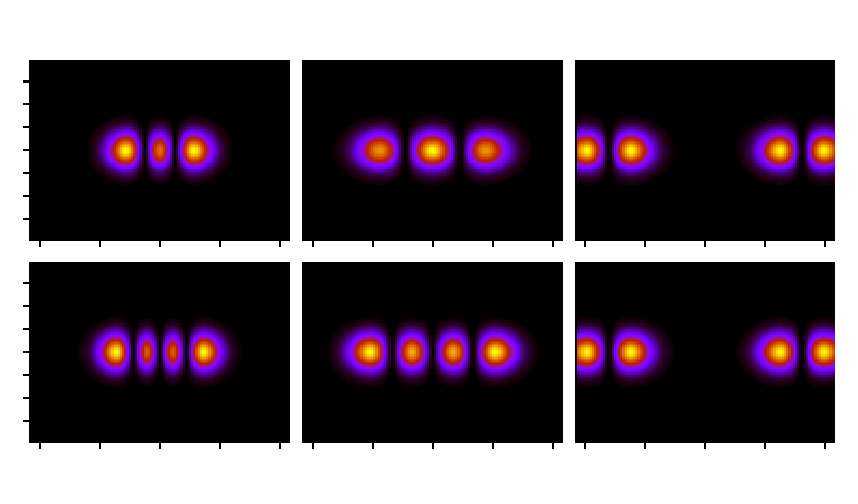
\includegraphics{images/phononProj2-3ir}}%
    \gplfronttext
  \end{picture}%
\endgroup

  \caption[Projection into phonon coordinates of the states with two and three infrared phonons.]
  {Projection into phonon coordinates of the states with two (top) and three (bottom) infrared phonons for three representative $\lambda_{ir}$ values.}
  \label{fig:phononProj2-3ir}
\end{figure}
